%%This is a very basic article template.
%%There is just one section and two subsections.
\documentclass{report}

%Included packages in alphabetical order (if dependencies do not prohibit)
\usepackage[english]{babel}
\usepackage{cite}

\usepackage{color}
\definecolor{lyellow}{rgb}{0.95,0.95,0.65}
\definecolor{morange}{rgb}{1,0.5,0.0}
\definecolor{mygreen}{rgb}{0,0.6,0}
\definecolor{mygray}{rgb}{0.5,0.5,0.5}
\definecolor{mymauve}{rgb}{0.58,0,0.82}

\usepackage{graphicx}
\usepackage[toc,acronyms,nosuper]{glossaries}

\usepackage{listings}
\lstset{ %
  backgroundcolor=\color{lyellow},   % choose the background color; you must add
  % \usepackage{color} or \usepackage{xcolor}; should come as last argument
  basicstyle=\footnotesize,        % the size of the fonts that are used for the code
  breakatwhitespace=false,         % sets if automatic breaks should only happen at whitespace
  breaklines=true,                 % sets automatic line breaking
  captionpos=b,                    % sets the caption-position to bottom
  commentstyle=\color{mygreen},    % comment style
  deletekeywords={...},            % if you want to delete keywords from the given language
  escapeinside={\%*}{*)},          % if you want to add LaTeX within your code
  extendedchars=true,              % lets you use non-ASCII characters; for 8-bits encodings only, does not work with UTF-8
  frame=single,	                   % adds a frame around the code
  keepspaces=true,                 % keeps spaces in text, useful for keeping indentation of code (possibly needs columns=flexible)
  keywordstyle=\color{blue},       % keyword style
  language=bash,                 % the language of the code
  morekeywords={*,...},            % if you want to add more keywords to the set
  numbers=left,                    % where to put the line-numbers; possible values are (none, left, right)
  numbersep=5pt,                   % how far the line-numbers are from the code
  numberstyle=\tiny\color{mygray}, % the style that is used for the line-numbers
  rulecolor=\color{black},         % if not set, the frame-color may be changed on line-breaks within not-black text (e.g. comments (green here))
  showspaces=false,                % show spaces everywhere adding particular underscores; it overrides 'showstringspaces'
  showstringspaces=false,          % underline spaces within strings only
  showtabs=false,                  % show tabs within strings adding particular underscores
  stepnumber=1,                    % the step between two line-numbers. If it's
  % 1, each line will be numbered
  stringstyle=\color{mymauve},     % string literal style
  tabsize=2,	                   % sets default tabsize to 2 spaces
  title=\lstname                   % show the filename of files included with \lstinputlisting; also try caption instead of title
}

\usepackage{multirow}
\usepackage{scrextend}


%shall be loaded close to last
\usepackage[hidelinks]{hyperref}


\begin{document}


%new commands
\newcommand{\fd}{\textit{FastDownward}}
\newcommand{\py}{\textit{Python}}
\newcommand{\cpp}{\textit{C++}}
\newcommand{\evaluate}{\textit{evaluate}}
\newcommand*{\fullref}[1]{\hyperref[{#1}]{\autoref*{#1} ``\nameref*{#1}''}}

\newenvironment{edit}[1]{\textbf{#1}\begin{addmargin}[0.5cm]{0.5cm}}{\end{addmargin}\ignorespacesafterend\bigskip}

%new acronyms
\newacronym{nn}{NN}{Neural Network}

\chapter{General \acrlong{nn} Framework}

Our first effort will be to implement a general framework to implement and
execute \gls{nn} experiments in \fd{}.

\section{Training-Evaluation Implementation}
Training Scheme:

\begin{lstlisting}[caption=Training Phase]
define/load network N
while some condition %*$C_T$*):
	sample training data (%*\fd*)) or load some data
	train network
	(Optionally) store network
store network and/or provide object pointer
\end{lstlisting}

\noindent{}Evaluation Scheme:
\begin{lstlisting}[caption=Evaluation Phase]
load network N/get pointer of N
while searching:
	# do search
	give state to N (convert format as necessary)
	obtain results (convert format as necessary)
	# continue search
\end{lstlisting}

\bigskip
\noindent{}For the training scheme i can imagine the following implementations:
\begin{table}[h]
\centering
\begin{tabular}{p{3cm}|p{2cm}|p{8cm}}	
Implementation & Advantages & Disadvantages\\\hline
In \fd{} (pure C++) & &
-good \cpp{} NN library?

-changing goal not supported now (on todo list)

-needs something encapsulating the training searches which is currently
not thought of now

-\fd{} initializes state space at start up, thus cannot be changed later
[on todo list]\\\hline

In \py{} (except \fd{} for sampling) & -many powerful libraries &
-slow data flow between \py{} and \fd{} (network serialization, training data)
[is intended to change by implementing a Python API, but before this can be
implemented, the todos in \fd{} disadvantages have to be solved]\\\hline
both & -maximal flexibility for user & -implement both version and solve all
problems of both versions
\end{tabular}
\caption{Advantages/Disadvantages of approaches}
\label{tbl-train-eval-scheme-adv-dis}
\end{table}


\noindent
\begin{edit}{Patrick}
I think we should plan on the implementation \textbf{both}, but start with the
\py{} version. The \cpp{} version cannot be done without major changes in \fd{}.
Although, in the last \fd{} meeting the idea for a Python API had positive
feedback and for this we would also do the here required reworks, I have no clue
how long this rework will take. The \py{} version can already be implemented. As
\py{} is today majorily used for deep learning, we have a huge arsenal of
libraries available and some should support also \cpp{} (see
\fullref{neural-network-libraries}). If it is implemented as new module to the
driver scripts of \fd{}, then the user does not feel a difference to a normal
\fd{} command (except for new arguments). A drawback is that the information
flow between \py{} and \cpp{} will be relatively slow compared to pure \cpp{}.
This might improve if the \py{} API is implemented, but still then there will be
an overhead for passing the objects around.

Thus, I think we should focus on the \py{} version, because we can already do
this, but when implementing it, we should already think on what the \cpp{} would
need. For example, the command line arguments should be the same such that the
user will not notice a difference and the sampling in \fd{} should support being
called from the outside (by \py{}) and from within (by the \cpp{} version).
\end{edit}



\section{Neural Network Libraries}
\label{neural-network-libraries}

\begin{table}[h]
\begin{tabular}{l|p{2cm}|l}
Name & Languages & Comments\\\hline
Tensorflow & \py{},\cpp & -training only in \py{} possible
\end{tabular}
\caption{Neuronal Network Libraries}
\label{tbl-neural-network-libraries}
\end{table}





\section{Neural Network Implementation}
\begin{edit}{Patrick}

The chosen training scheme restricts our freedom of library choices, but still
multiple libraries might be possible. I suggest structuring the code in \fd{}
in such a way that it can be extended for any library. A possible structure can
be seen in \autoref{fig-uml-fd-nn}.

An abstract \gls{nn} base class provides the \evaluate{} method which takes as
input the data provided by \fd{} for a state evaluation. A library should
subclass this and implement its own management parts. The example shows a class
for Protobuf (which is the format used by tensorflow to store graphs). A
concrete \gls{nn} usable by the user would subclass the base class of its
library. \Glspl{nn} can output very different things, thus, the networks
\evaluate{} does not return anything, but instead it shall set member variables.
A concrete network implements then some interfaces for the output it produces
(it might produce multiple different outputs) and his interface methods shall
provide access to the output of the \gls{nn} associated to the interface (e.g.
a heuristic value). New interfaces can be added for new kinds of output of
\glspl{nn}.
\end{edit}
%\usepackage{graphics} is needed for \includegraphics

\begin{figure}[ht]
\vspace*{-7cm}
\begin{center}
	%\hspace*{-5cm}
	%\vspace*{-5cm}
  \centerline{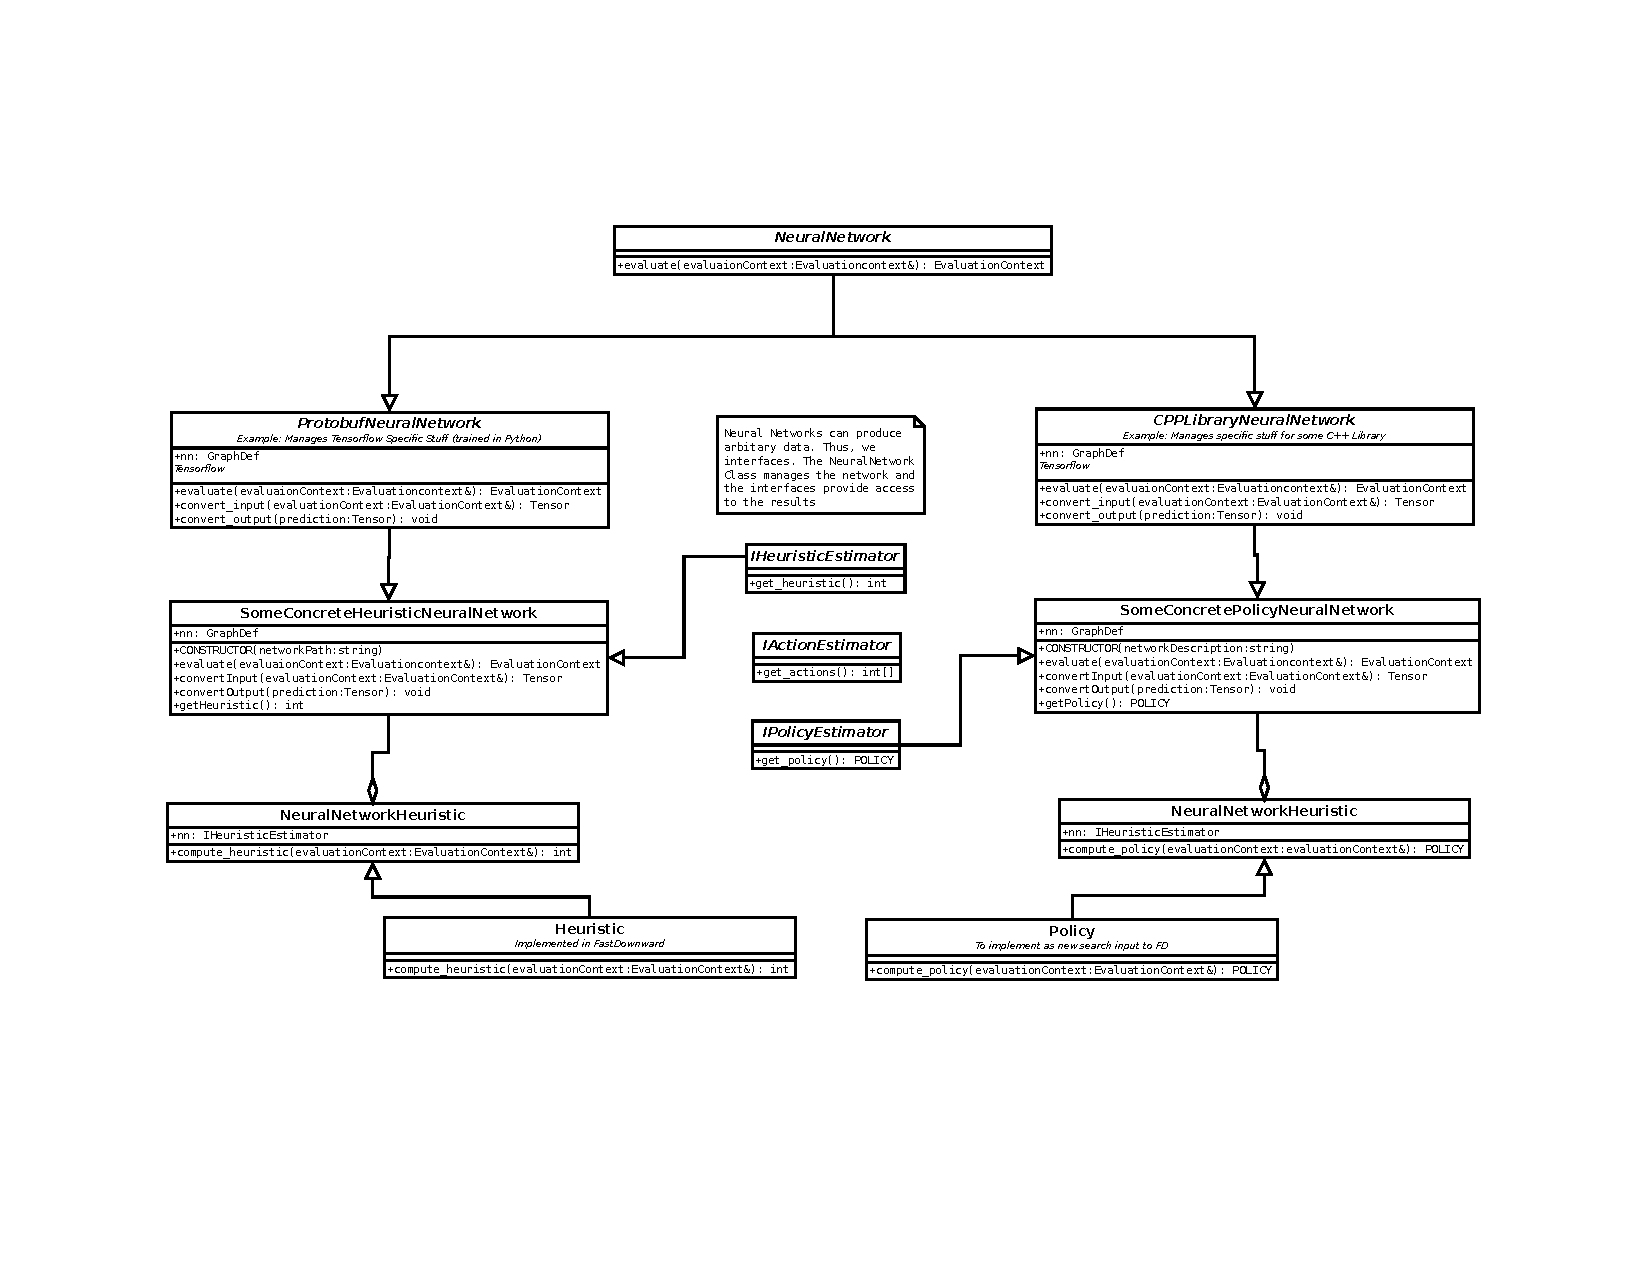
\includegraphics[width=2.5\textwidth,
  angle=270]{images/UML_FD_NN}}
  \caption{UML Diagram of \gls{nn} implementation in \fd{}}
  \label{fig-uml-fd-nn}
\end{center}
\end{figure}



\section{Policies}
A new thing we might want to implement in \fd{} would be policies. A policy
tells the search which actions to choose in a state together with a rating for
the action.

{\color{morange} Are Preferred Operators policies with equal rating among
all chosen actions?}

Most times \glspl{nn} which output an action to chose actually output actions
with a rating, therefore, could be directly used as policy.
\end{document}
